\section{Estatísticas}

Para efeitos estatíscos apresentamos duas opções para o utilizador:

\begin{enumerate}
  \item Descoberta da personalidade que mais apereceu nas notícias extraídas;
  \item Dado um nome de uma personalidade devolvemos o número de vezes que esta apareceu nas notícias.
\end{enumerate}

O procecidemento para desenvolver os tópicos atrás enumerados, foi uma simples contagem dos elementos presentes na base de dados. Em baixo, apresentamos alguns gráficos que representam o número de vezes que uma certa personalidade apareceu nas notícias num determinado dia.

\begin{figure}[htbp]
  \centering
    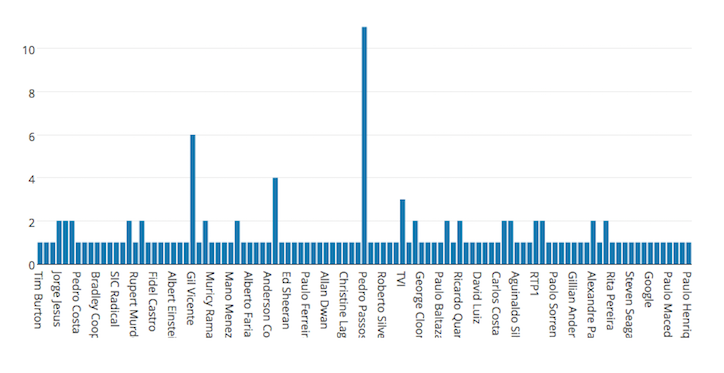
\includegraphics[width=0.9\textwidth]{images/day_one.png}
	\caption{Personalidades no dia 9 de maio de 2015}
\end{figure}

\begin{figure}[htbp]
  \centering
    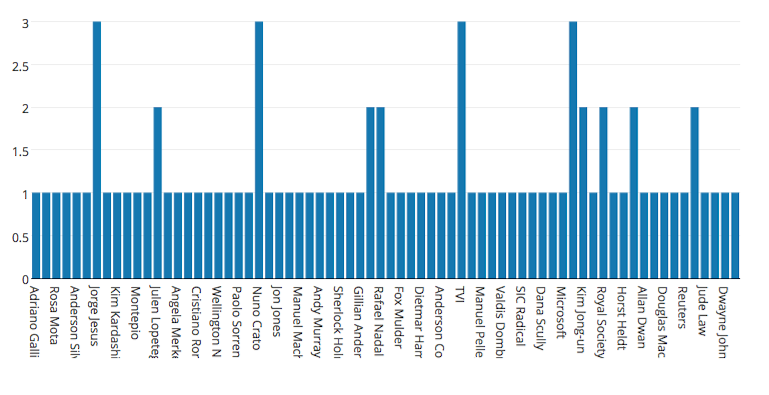
\includegraphics[width=0.9\textwidth]{images/day_two.png}
	\caption{Personalidades no dia 13 de maio de 2015}
\end{figure}

\begin{figure}[htbp]
    \centering
    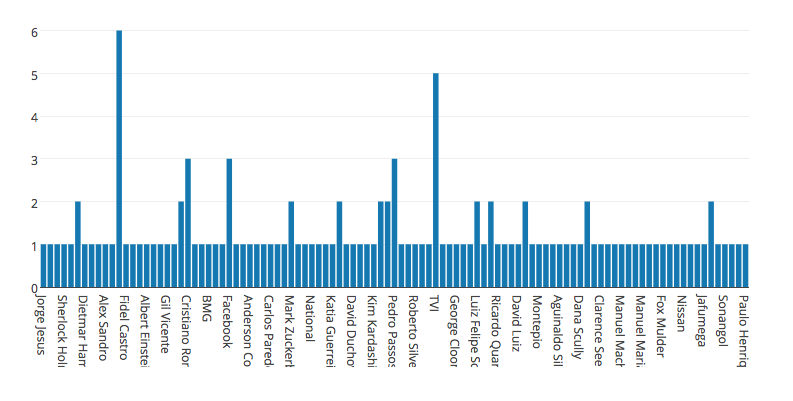
\includegraphics[width=1\textwidth]{images/search55.png} %trocar para imagem do dia 14 ou 15 de maio
    \caption{Personalidades no dia 14 de maio de 2015}
\end{figure}

